\newpage
\section{Conception et mise en œuvre}
\label{sec:impl}
\subsection{Architecture globale du logiciel}

On a choisi une architecture \textbf{MVC (Modèle-Vue-Contrôleur)} pour bien séparer le moteur de jeu de l'interface graphique. Cette séparation nous a permis de travailler plus facilement en équipe et de tester chaque partie indépendamment.

\begin{itemize}
\item \textbf{Modèle} : les packages \texttt{engine.map} et \texttt{engine.mobile} gèrent le plateau et les pièces ;
\item \textbf{Contrôleur} : le package \texttt{engine.process} gère la logique du jeu et le bot ;
\item \textbf{Vue} : le package \texttt{gui} s'occupe de tout l'affichage avec Java Swing.
\end{itemize}

\begin{figure}[H]
\centering
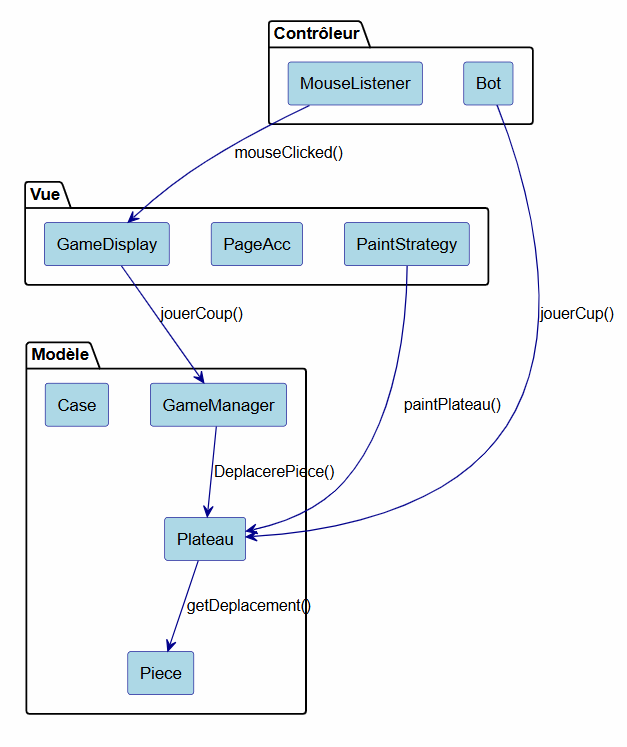
\includegraphics[width=12cm, height=12cm]{images/diagrammeMVC.png}
\caption{Architecture MVC du projet }
\label{fig:accueil1}
\end{figure}

\subsection{Packages }
\paragraph{} Voici la structure complète des packages du projet :
\begin{itemize}
\item \texttt{config} : constantes globales comme la taille du plateau et des cases ;
\item \texttt{engine.map} : contient \texttt{Plateau}, \texttt{Case}, \texttt{CaseNormal}, \texttt{CaseMort}, \texttt{Couleur}, \texttt{TypeCaseNormale} ;
\item \texttt{engine.mobile} : contient la classe abstraite \texttt{Piece} et ses sous-classes \texttt{General}, \texttt{Conseillere}, \texttt{Elephant}, \texttt{Chevalier}, \texttt{Char}, \texttt{Canon}, \texttt{Soldat} ;
\item \texttt{engine.process} : contient \texttt{GameManager}, \texttt{Bot}, \texttt{Coup}, \texttt{Niveau} ;
\item \texttt{gui} : contient \texttt{MainGUI}, \texttt{PageAcc}, \texttt{GameDisplay}, \texttt{PaintStrategy} ;
\item \texttt{log} : configuration des logs avec Log4j ;
\item \texttt{junit} : tests unitaires avec JUnit.
\end{itemize}
%\begin{figure}
%\centering
%\includegraphics[width=3.5cm, height=2cm]{images/architecture.png}
%\caption{Architecture MVC du projet}
%\label{fig:architecture}
%\end{figure}


\subsection{Classes de données}
\begin{figure}[H]
\centering
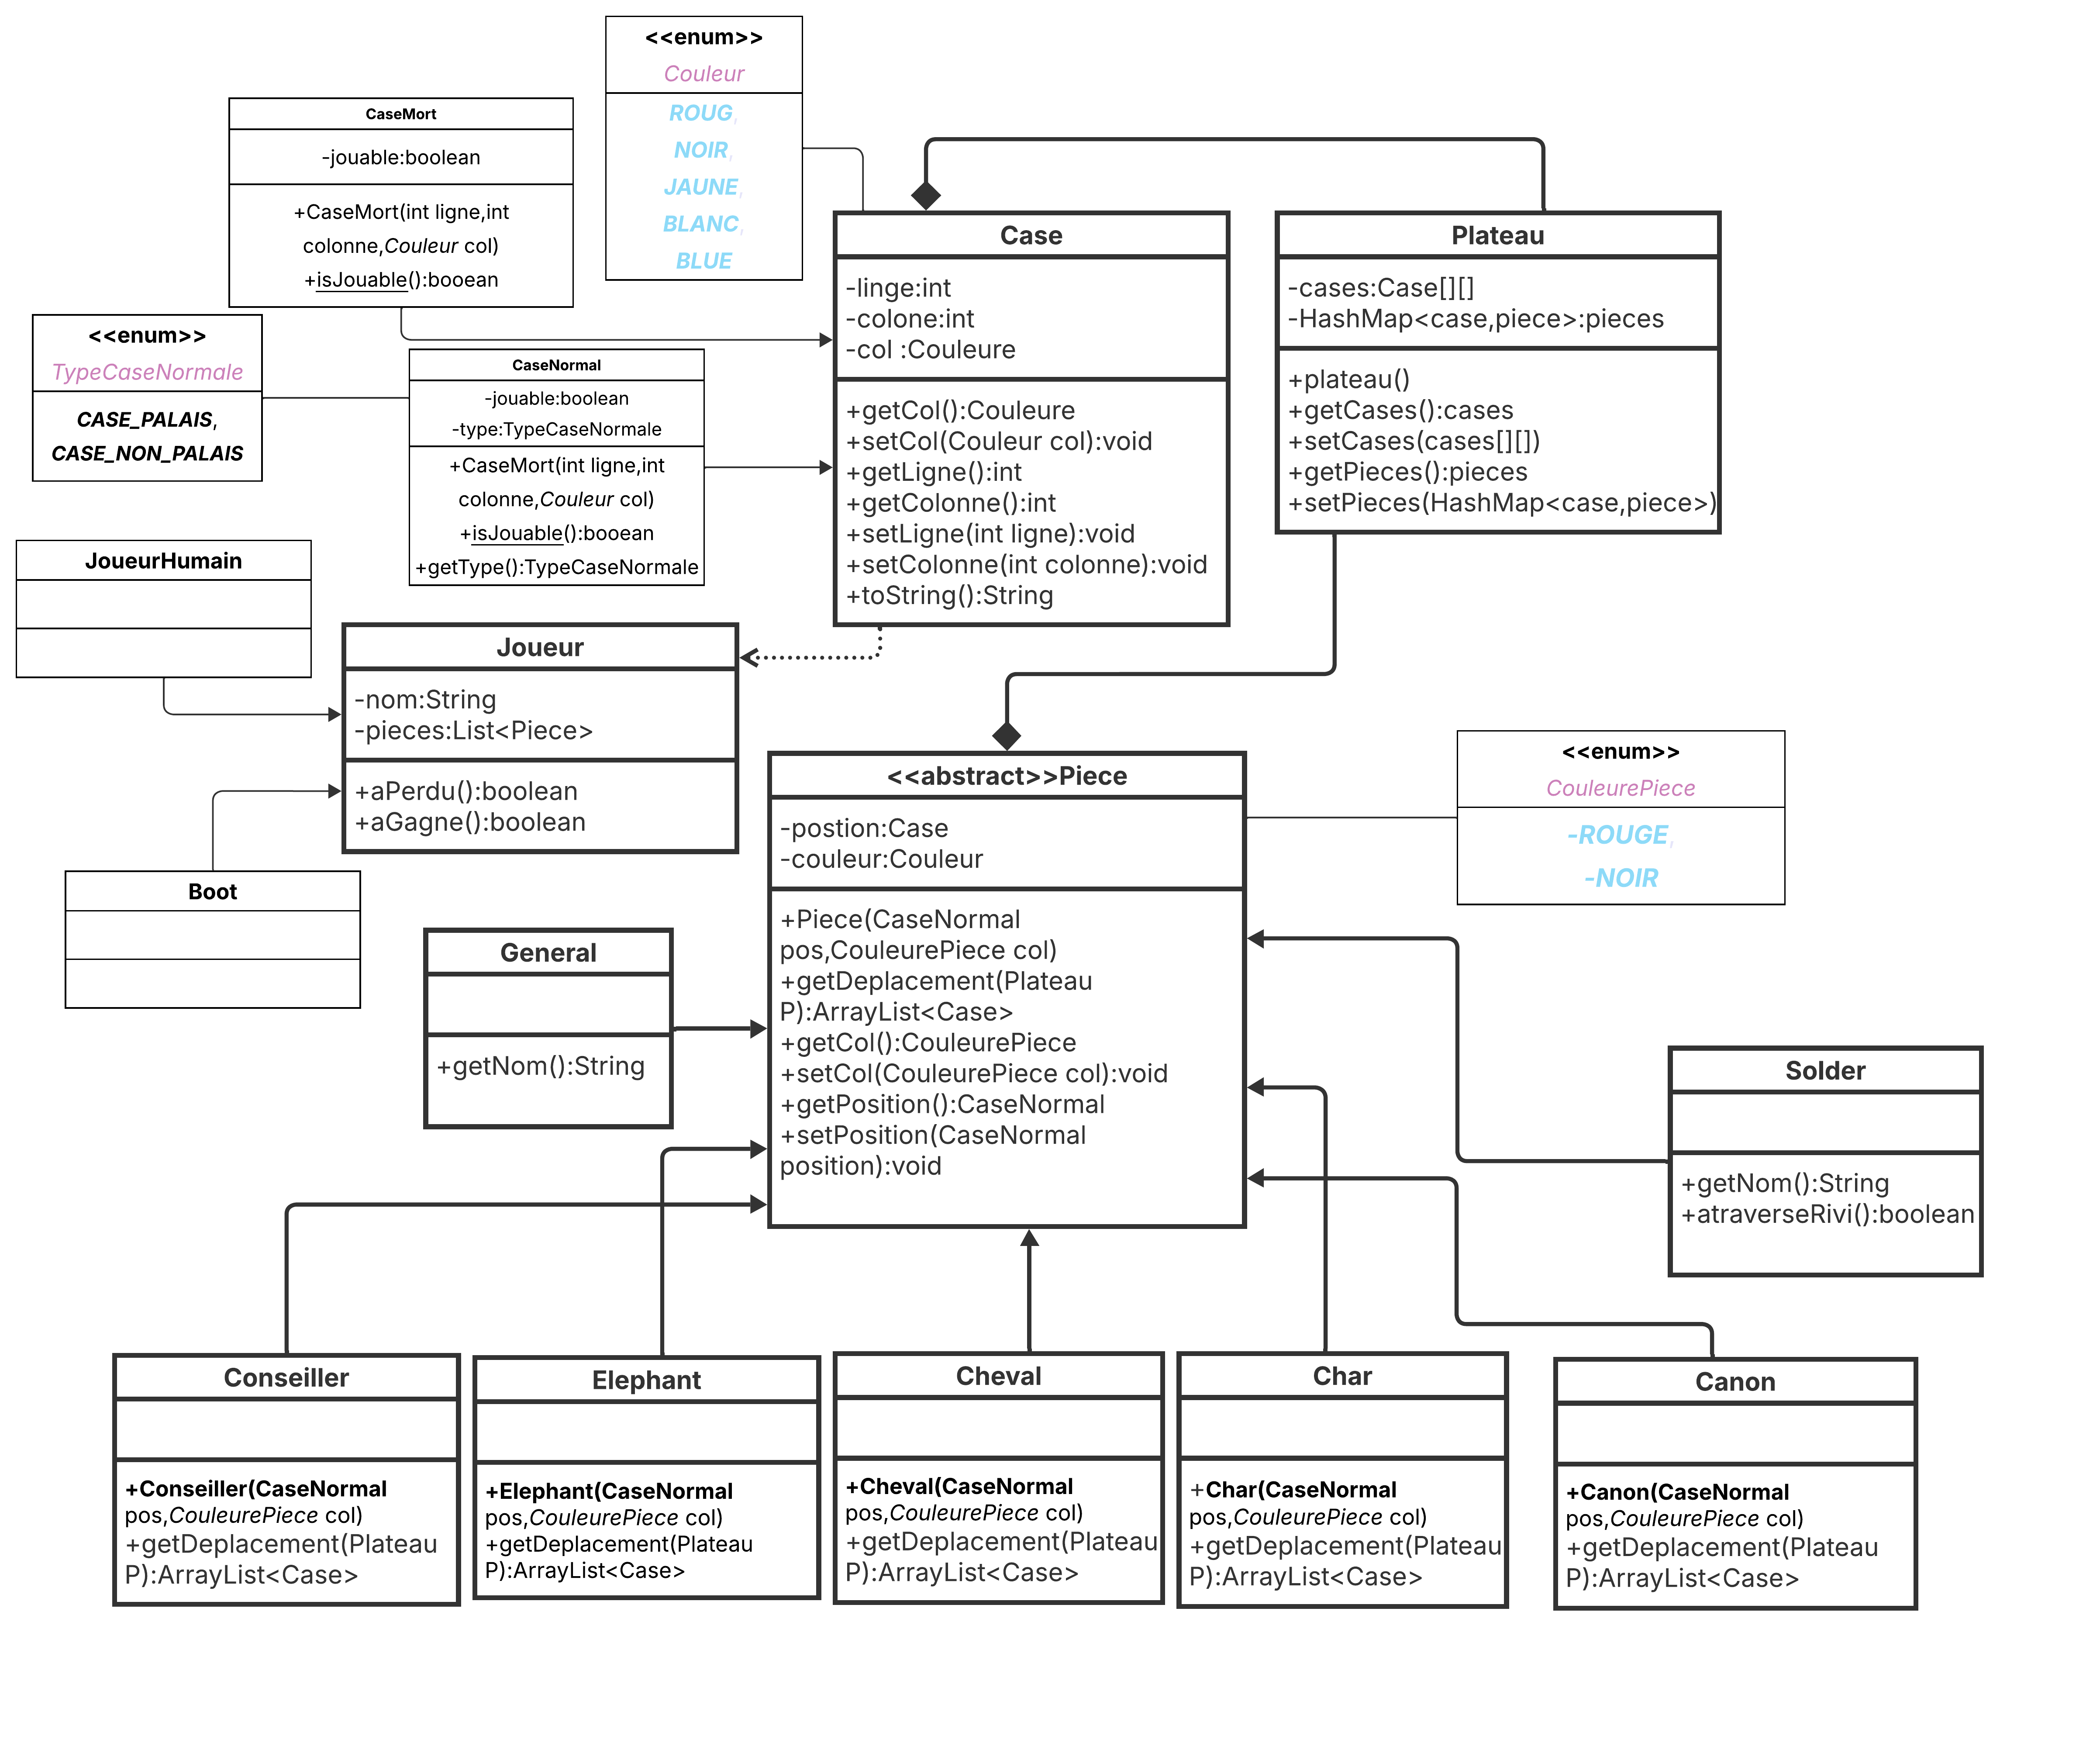
\includegraphics[width=16cm, height=14cm]{images/diagrammeclasses.png}
\caption{Diagramme de classes }
\label{fig:accueil2}
\end{figure} 


\subsubsection{La classe Plateau}
\paragraph{} La classe Plateau est au cœur du projet. Elle représente l'état complet du jeu à tout moment. Elle contient :
\begin{itemize}
\item un tableau \texttt{Case[11][11]} qui représente la grille du plateau ;
\item une \texttt{HashMap<Case, Piece>} qui associe chaque case occupée à sa pièce ;
\item la couleur du joueur dont c'est le tour (\texttt{CouleurePiece}) ;
\item deux listes pour stocker les pièces capturées (une par couleur).
\end{itemize}
\subsubsection{Initialisation du plateau}
\paragraph{} Au démarrage, les cases neutres (colonnes 3 et 7) et la rivière (ligne 5) sont initialisées comme des \texttt{CaseMort}. Les cases du palais sont de type \texttt{CASE\_PALAIS}.
\subsubsection{Méthodes principales}
\paragraph{} Les méthodes les plus importantes de \texttt{Plateau} sont :
\begin{itemize}
\item \texttt{coupValide(depart, arrivee)} : simule un coup et vérifie que le Général n'est pas en échec et qu'il n'y a pas de face à face après le coup ;
\item \texttt{estMenacer(case, couleur)} : vérifie si une case est attaquée par une couleur donnée ;
\item \texttt{EnEchec(joueur)} : dit si un joueur est actuellement en échec ;
\item \texttt{EnEchecEtMat(joueur)} : vérifie si un joueur n'a plus aucun coup légal ;
\item \texttt{RoiFacAfac()} : détecte si les deux Généraux sont sur la même colonne sans pièce entre eux.
\end{itemize}
\subsubsection{La hiérarchie des pièces}
\paragraph{} La classe abstraite \texttt{Piece} définit la méthode \texttt{getDeplacement(Plateau)} que chaque sous-classe redéfinit selon ses propres règles. Par exemple, le \texttt{Canon} parcourt les cases horizontalement et verticalement en ignorant les colonnes neutres, et cherche un écran avant de pouvoir capturer.



\subsection{IHM Graphique}
\paragraph{} L'interface graphique est faite avec \textbf{Java Swing} et est composée de trois classes principales :
\begin{itemize}
\item \texttt{PageAcc} : la page d'accueil avec un fond d'image, le titre du jeu, et les boutons pour choisir le mode de jeu. En mode VS BOT, un second dialogue apparaît pour choisir la difficulté ;
\item \texttt{GameDisplay} : le panneau principal pendant la partie. Il contient le plateau au centre, les zones de captures en haut et en bas, et un panneau à droite avec l'historique des coups et le bouton menu ;
\item \texttt{PaintStrategy} : s'occupe uniquement du rendu graphique — dessine les cases, les pièces (images PNG) et les surbrillances des coups légaux.
\end{itemize}
\subsection{Conception des traitements (processus)}

\subsubsection{Diagramme de sequence}
\begin{figure}[H]
\centering
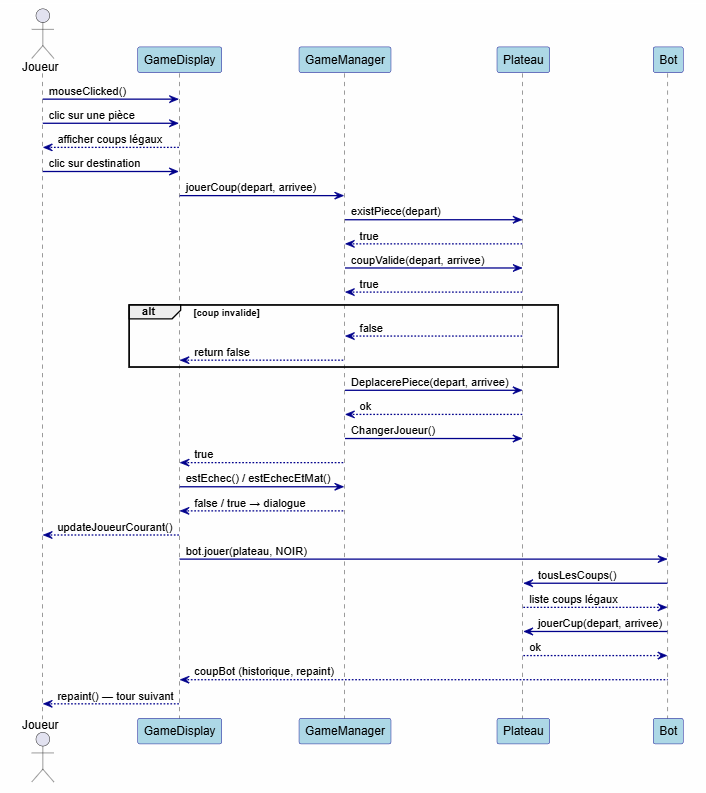
\includegraphics[width=15cm, height=15cm]{images/diagrammesequence.png}
\label{fig:accueil3}
\end{figure}

\subsubsection{Les niveaux du bot}
\paragraph{} Le bot dispose de trois niveaux définis dans l'énumération \texttt{Niveau} :
\begin{itemize}
\item \textbf{Facile} : le bot choisit un coup au hasard parmi tous ses coups légaux ;
\item \textbf{Moyen} : le bot essaie de capturer la pièce adverse la plus précieuse, en vérifiant d'abord que la case d'arrivée n'est pas dangereuse pour lui ;
\item \textbf{Difficile} : le bot calcule un score pour chaque coup possible. Ce score prend en compte la valeur de la pièce capturée, le danger pour ses propres pièces, la mise en échec de l'adversaire et la sécurité de son Général.
\end{itemize}
\paragraph{} Le tableau \ref{tab:valeurs} montre les valeurs utilisées par le bot pour évaluer les pièces.

\begin{table}[H]
\centering
\begin{tabular} {|p{3.5cm}|p{2cm}|}
\hline
\textbf{Pièce} & \textbf{Valeur} \\
\hline
Général & 100 \\
\hline
Chariot & 9 \\
\hline
Canon & 5 \\
\hline
Chevalier & 4 \\
\hline
Éléphant & 3 \\
\hline
Conseillère & 2 \\
\hline
Soldat & 1 \\
\hline
\end{tabular}
\caption{Valeurs des pièces utilisées par le bot}
\label{tab:valeurs}
\end{table}

\subsubsection{Validation des coups}
\paragraph{} Dans l'algorithme1, on décrit comment un coup est validé avant d'être joué.

\begin{algorithm}[H]
\caption{Validation d'un coup avant de jouer}
\label{algo:valide}
\begin{algorithmic}
\REQUIRE Départ $d$, Arrivée $a$, Plateau $P$
\ENSURE Vrai si le coup est légal, Faux sinon
\IF{$a \notin$ getDeplacement($d$, $P$)}
    \RETURN Faux
\ENDIF
\STATE Simuler : déplacer la pièce de $d$ vers $a$
\IF{le Général du joueur courant est menacé}
    \RETURN Faux
\ENDIF
\IF{les deux Généraux sont face à face}
    \RETURN Faux
\ENDIF
\STATE Annuler la simulation
\RETURN Vrai
\end{algorithmic}
\end{algorithm}
%%% Une autre façon pour écrire un algorithme %%%
%\begin{algorithm}[H]
 %\KwData{this text}
 %\KwResult{how to write algorithm with \LaTeX2e }
 %initialization\;
 %\While{not at end of this document}{
  %read current\;
  %\eIf{understand}{
   %go to next section\;
   %current section becomes this one\;
   %}{
   %go back to the beginning of current section\;
  %}
 %}
 %\caption{How to write algorithms}
%\end{algorithm}

\subsubsection{Tests unitaires}
\paragraph{} Les tests unitaires sont dans la classe \texttt{PlateauTest} et utilisent JUnit. On a testé les cas suivants :
\begin{itemize}
\item Le plateau et les pièces sont bien initialisés au démarrage ;
\item Le premier joueur est bien ROUGE ;
\item Le changement de joueur fonctionne correctement après un coup ;
\item La détection de présence ou d'absence de pièce sur une case ;
\item Un coup valide est bien accepté, un coup invalide est bien refusé ;
\item La détection des cases de bordure ;
\item Les deux Généraux sont bien présents sur le plateau ;
\item Aucun joueur n'est en échec au début de la partie ;
\item Une capture est bien enregistrée dans la liste correspondante ;
\item Les Généraux ne sont pas face à face en position initiale.
\end{itemize}

